\documentclass[
    10pt,
    aspectratio=169,
    xcolor={dvipsnames},
    spanish,
    % handout,
    % notes=only,
    % notes,
    ]{beamer}

% BEAMER SETTINGS
\setbeamerfont{section in toc}{size=\normalsize, shape=\bfseries}
\mode<presentation>{
    \usetheme{Antibes}
    \setbeamercovered{transparent}
    \usecolortheme{rose}
    \setbeamertemplate{navigation symbols}{}
    }

% PACKAGES
% \usepackage[spanish]{babel}  % uncomment for Spanish support
\usepackage{tikz,pgfplots}
\pgfplotsset{compat=1.13}
\usetikzlibrary{calc}
\usepackage{subcaption}
\usepackage{graphicx}
\graphicspath{{figures}}
\usepackage{booktabs}
\usepackage{upgreek}
\usepackage{commath}
\usepackage{amsmath,amsthm,amssymb,mathtools,mathrsfs}
\usepackage{cancel}
\usepackage{fontawesome5}
\usepackage{enumerate}
\usepackage{tensor}
\usepackage[font=footnotesize]{caption}
\usepackage{wasysym}

\usepackage[skins,theorems]{tcolorbox}
\tcbset{
    highlight math style={
        enhanced,
        coltext=black,
        colframe=black,
        colback=lightgray,
        arc=0pt,
        boxrule=.5pt
        }
}

% REFERENCES AND OTHERS
\usepackage{aas_macros}
\usepackage{natbib}
\bibpunct{(}{)}{;}{a}{}{,}

\usepackage{siunitx}
\sisetup{
    range-phrase=\text{--},
    range-units=single,
    separate-uncertainty=true,
    print-unity-mantissa=false
    }
\DeclareSIUnit{\gauss}{G}
\DeclareSIUnit{\jansky}{Jy}
\renewcommand{\figurename}{Fig.}

\usepackage{hyperref}
\hypersetup{
    % bookmarks=true,
    unicode=true,
    pdftoolbar=true,
    pdfmenubar=true,
    pdffitwindow=false,
    pdfstartview={FitH},
    pdftitle={ISI-Free Linear Combination Pulses with Better Performanc},
    pdfauthor={Erik Saez A.},
    pdfcreator={Erik Saez A.},
    pdfnewwindow=true,
    colorlinks=true,
    linkcolor=RoyalBlue,
    citecolor=RoyalBlue,
    urlcolor=RoyalBlue
    }

\title[Auxiliar \#4 - Ondas ondas ondas]{\bfseries Auxiliar \#4 - Ondas ondas ondas}
\subtitle{Introducción a la Física Moderna (F1100-5)}
\author[Erik Saez A.]{Erik Saez A. - Javiera Toro}
\institute[UChile]{Departamento de Ingeniería Eléctrica \\ Universidad de Chile}

\date{\today}

\begin{document}

\begin{frame}
  \titlepage
  \centering
  \faIcon{envelope} \href{mailto:erik.saez@ug.uchile.cl}{erik.saez@ug.uchile.cl} \hspace{.2cm}
\end{frame}

\begin{frame}{Contenidos}
  \tableofcontents
\end{frame}

\section{Resumen}

\begin{frame}{Resumen: Oscilador forzado (bloque–resorte)}
  \footnotesize
  \begin{block}{Cambio de variable y EDO}
  Para un bloque de masa $m$ colgando de un resorte ($k$, $\ell_0$) con techo móvil $y_t=A\cos(\Omega t)$, usando
  \[ z= y-\ell_0-\tfrac{mg}{k} \]
  \vspace{-6pt}
    se obtiene el oscilador forzado sin amortiguamiento
    \[ \ddot z + \omega^2 z = \omega^2 A\cos(\Omega t),\qquad \omega^2=\tfrac{k}{m}. \]
  \end{block}
  \begin{block}{Solución útil}
    Respuesta estacionaria: amplitud \( B=\dfrac{\omega^2 A}{\omega^2-\Omega^2} \). En resonancia ($\Omega=\omega$) crece linealmente en el tiempo. La coordenada original: \( y(t)=z(t)+\ell_0+\tfrac{mg}{k} \).
  \end{block}
\end{frame}

% =====================================
\begin{frame}{Resumen: Ondas en cuerda y onda estacionaria}
  \footnotesize
  \begin{columns}[T]
    \begin{column}{0.57\textwidth}
      \begin{block}{Onda viajera y rapidez}
        Rapidez \( c=\sqrt{T/\rho} \), número de onda \( k=\omega/c \). Ansatz de superposición:
        \[ y=A\sin(kx-\omega t)+B\sin(kx+\omega t). \]
      \end{block}
      \begin{block}{Forma de onda estacionaria}
        Usando identidades trigonométricas:
        \[
          y=(A+B)\,\sin(kx)\cos(\omega t)+(B-A)\,\cos(kx)\sin(\omega t).
        \]
      \end{block}
    \end{column}
    \begin{column}{0.4\textwidth}
      %\centering
      %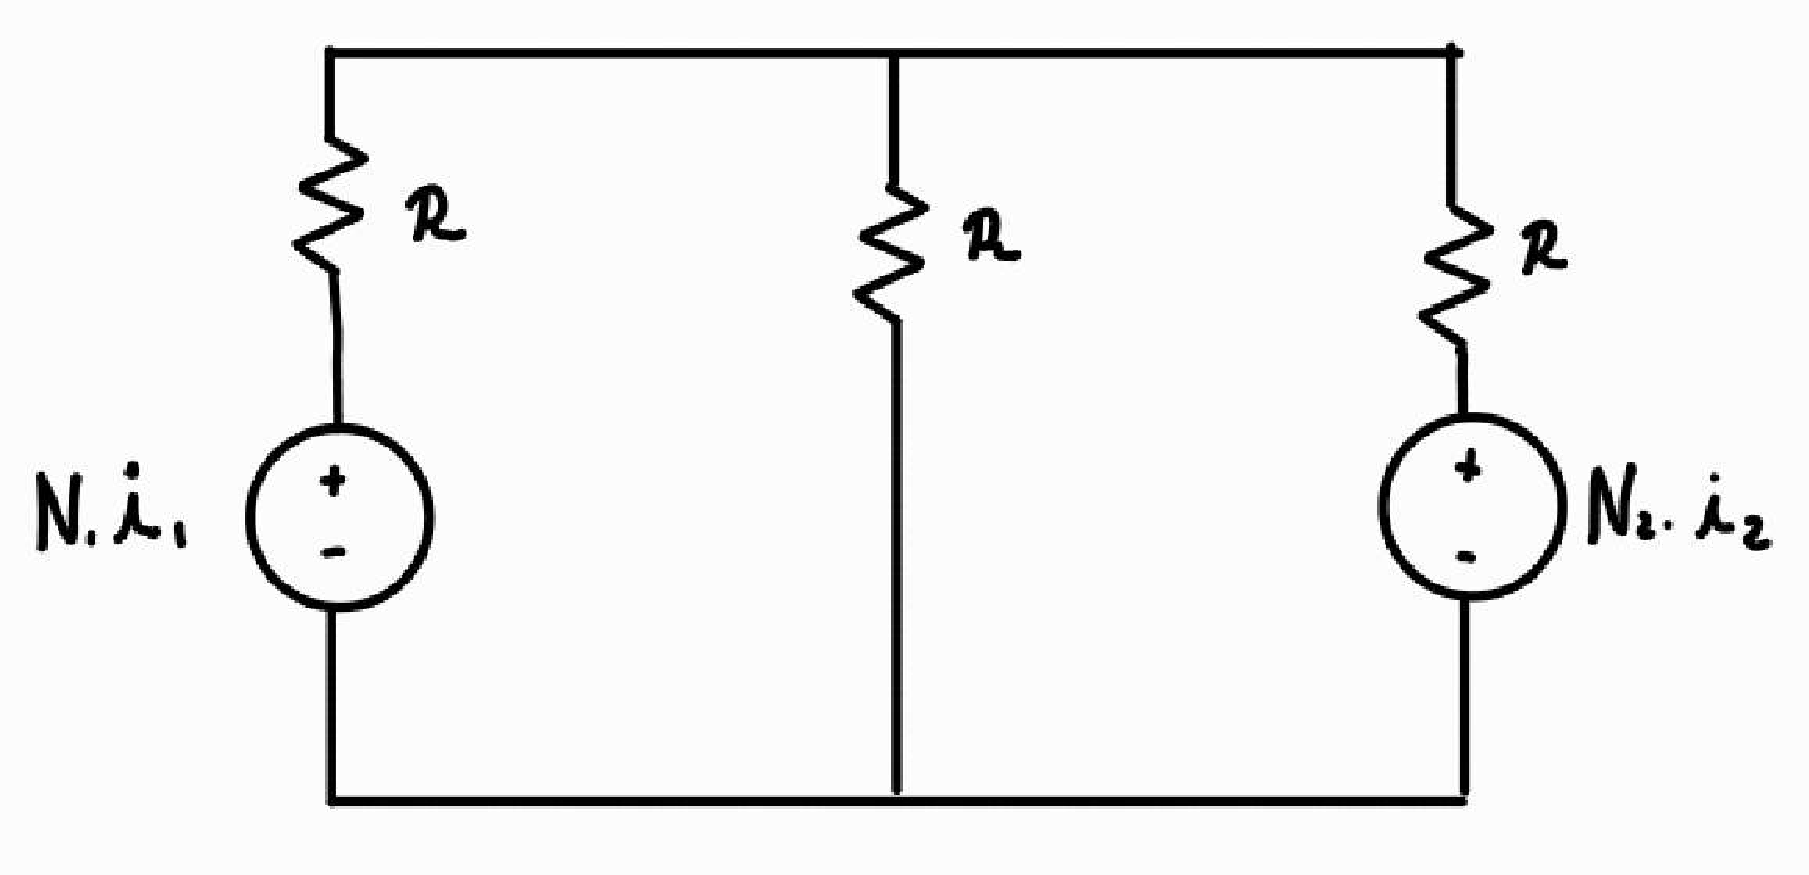
\includegraphics[width=.95\linewidth]{Auxiliar_2_2}
    \end{column}
  \end{columns}
\end{frame}

\begin{frame}{Condiciones de borde usadas hoy}
  \footnotesize
  \begin{itemize}
    \item Extremos fijos: $y(0,t)=y(L,t)=0$ $\Rightarrow$ $k=\dfrac{n\pi}{L}$, $n=1,2,\dots$
    \item Extremos con aceleración impuesta: $\ddot y(0,t)=\ddot y(L,t)=a_0\sin(\Omega t)$.
    \begin{itemize}
      \item Con la ansatz anterior: $\Omega=\omega$ y $\cos(kL)=1\;\Rightarrow\;kL=2\pi n$.
      \item En régimen forzado puro: $y(x,t)= -\dfrac{a_0}{\omega^2}\cos(kx)\sin(\omega t)$.
    \end{itemize}
    \item Velocidad en el punto medio (extremos fijos): $\left.\partial_t y\right|_{x=L/2}=v_0\sin(\Omega t)$.
    \begin{itemize}
      \item Se exige $A=B$ y solo se excitan \textbf{modos impares} $n=1,3,5,\dots$
      \item $y_n(x,t)= -\dfrac{v_0}{\Omega}(-1)^{\frac{n-1}{2}}\sin\!\left(\dfrac{n\pi}{L}x\right)\cos(\Omega t)$.
    \end{itemize}
  \end{itemize}
\end{frame}

\begin{frame}{Cuerda colgante y reflexiones}
  \footnotesize
  \begin{itemize}
    \item Tensión variable: $T(z)=\rho g\,z \;\Rightarrow\; c(z)=\sqrt{g z}$ (mayor rapidez hacia arriba).
    \item El pulso que sube llega primero al techo (extremo fijo) y se \textbf{invierte}; el que baja llega al extremo libre y \textbf{no} se invierte.
    \item Se reencuentran \textbf{por debajo del centro} y con signos opuestos $\Rightarrow$ \textbf{interferencia destructiva}.
  \end{itemize}
\end{frame}

\begin{frame}{Cavidad acústica (túnel)}
  \footnotesize
  \begin{itemize}
    \item Modelo \emph{abierto–cerrado} $\Rightarrow$ solo \textbf{modos impares}: $f_n=\dfrac{(2n+1)c}{4L}$.
    \item Espaciamiento entre resonancias consecutivas: $\Delta f=\dfrac{c}{2L}\;\Rightarrow\; L=\dfrac{c}{2\,\Delta f}$.
    \item Con $c=335\,\text{m/s}$ y $f=4.5,\;6.3\,\text{Hz}$, $\Delta f=1.8\,$Hz $\Rightarrow$ $L\approx 93\,$m.
  \end{itemize}
\end{frame}
% ===================================

% =====================================
\section{Pregunta 1}

% ------------------ Ejercicio 1 ------------------
\begin{frame}{Ejercicio 1: Corcho flotante}
  \begin{columns}[T,totalwidth=\textwidth]
    \begin{column}{0.60\textwidth}
      \begin{block}{Enunciado pregunta 1}
        Corcho cilíndrico de radio $R$ y altura $H$ se deja en una piscina en reposo hasta alcanzar su posición de equilibrio.
        \begin{itemize}
          \item Calcular la posición de equilibrio.
          \item Si se perturba ligeramente y en $t=0$ está en $x_0$ con velocidad $v_0$, hallar $x(t)$.
        \end{itemize}
        Datos: gravedad $g$ y fuerza de empuje $F_e=\rho g V$, con $\rho$ densidad del agua y $V$ volumen sumergido.
      \end{block}
    \end{column}
    \begin{column}{0.40\textwidth}
      \centering
       \vspace*{1cm}
      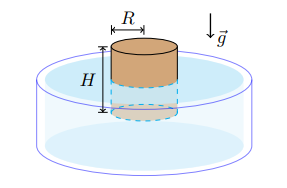
\includegraphics[width=0.9\textwidth]{Auxiliar_1_1 copy.png}
    \end{column}
  \end{columns}
\end{frame}
\section{Pregunta 2}
% ------------------ Ejercicio 2 ------------------
\begin{frame}{Ejercicio 2: Masa entre dos resortes}
  \begin{block}{Enunciado pregunta 2}
    Bloque de masa $M$ entre dos resortes ideales de constantes $k$ y $2k$ (longitudes naturales nulas), sin fricción, movimiento 1D. Inicialmente en equilibrio con velocidad $V$ hacia la derecha.
    \begin{itemize}
      \item Frecuencia angular $\omega$ y amplitud.
      \item Expresión de $x(t)$.
      \item Al cortarse el resorte derecho en su máxima elongación, tiempo hasta el choque con la pared izquierda.
    \end{itemize}
  \end{block}
  \vspace{2pt}
  \centering
  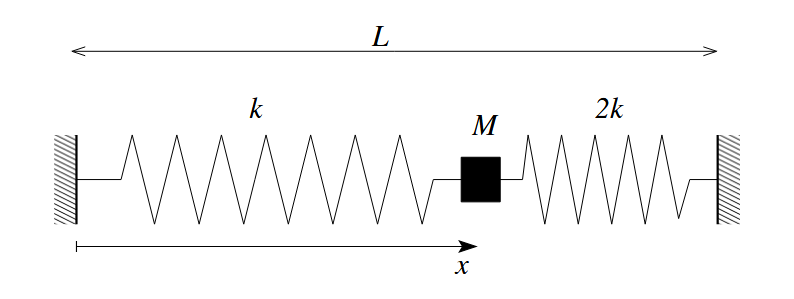
\includegraphics[width=0.6\textwidth]{Auxiliar_1_2 copy.png}
\end{frame}
\section{Pregunta 3}
% ------------------ Ejercicio 3 ------------------
\begin{frame}{Ejercicio 3: Cavidad óptica}
  \footnotesize
  \begin{columns}[T,totalwidth=\textwidth]
    \begin{column}{0.55\textwidth}
      \begin{block}{Enunciado Pregunta 3}
        Una cavidad óptica, elemento básico para construir un láser, puede hacerse usando un espejo plano (Espejo 1) y uno esférico cóncavo (Espejo 2), como en la figura.
        \begin{enumerate}
          \item Con $s_1=5\,\mathrm{m}$, $s_2=20\,\mathrm{m}$, $R=10\,\mathrm{m}$ y altura del peón $h_1=5\,\mathrm{cm}$, determine las imágenes del peón por ambos espejos: si son reales/virtuales, invertidas/derechas y su tamaño.
          \item Use estas dos imágenes como nuevos objetos para generar dos nuevas imágenes; repita el razonamiento para explicar por qué aparecen infinitas imágenes al enfrentar dos espejos.
        \end{enumerate}
      \end{block}
    \end{column}
    \begin{column}{0.40\textwidth}
      \centering
  % bajar solo la imagen de la Pregunta 3
  \vspace*{1cm}
      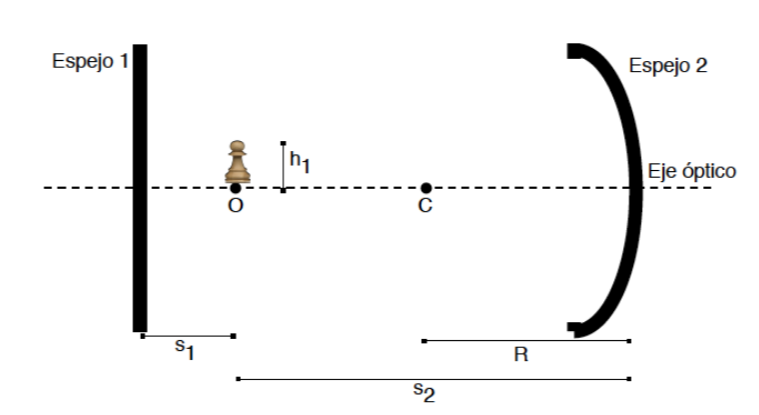
\includegraphics[width=1\textwidth]{Auxiliar_1_5 copy.png}
    \end{column}
  \end{columns}
\end{frame}

\end{document}
